\documentclass[dvipdfmx, titlepage, 11pt]{jsarticle}
\usepackage{tikz}
\usetikzlibrary{patterns}
\usetikzlibrary{intersections,calc,arrows}
\usepackage[top=20truemm,bottom=20truemm,left=15truemm,right=15truemm]{geometry}
\usepackage{enumerate}
\usepackage{multicol}
\usepackage{diagbox}
\usepackage{graphicx}

\makeatletter
\newcommand{\overarc}[1]{
  \setbox0\hbox{#1}%
  \ifdim\wd0<1em%
    \stackrel{\frown}{#1}%
  \else\ifdim\wd0<1.75em%
    \stackrel{\rotatebox{90}{\big)}}{#1}%
  \else\ifdim\wd0<2.5em%
    \stackrel{\rotatebox{90}{\Big)}}{#1}%
  \else\ifdim\wd0<3.25em%
    \stackrel{\rotatebox{90}{\bigg)}}{#1}%
  \else%
    \stackrel{%
      \rotatebox[origin=c]{90}{\mbox{%
        $\left.\vphantom{\rotatebox[origin=c]{90}{#1}}\right)$%
      }}%
    }{#1}%
  \fi\fi\fi\fi%
}
\makeatother

\newcommand{\ncircle}[1]{\textcircled{\scriptsize #1}}
\newcommand{\nbox}[1]{\fbox{\hspace{5pt} \textcircled{\scriptsize #1}\hspace{5pt} }}
\newcommand{\ebox}{\fbox{ \hspace{10pt} }}

\title{\Huge 数学}
\author{\LARGE 試験時間 : 50分}
\date{\LARGE 平成29年度筑波大附属高校\\[3cm] 大問は \fbox{\Large {\bf 1}} から \fbox{\Large {\bf 5}} まであります\\[0.5cm] 解答は解答用紙に記入して下さい}
\begin{document}
\maketitle

\newpage
\thispagestyle{empty}
 
\newpage

\newpage
\thispagestyle{empty}
 
\newpage

\setcounter{page}{1}
\noindent \fbox{\LARGE {\bf 1}}\hspace{10pt} 次の\textcircled{\scriptsize 1} 〜 \textcircled{\scriptsize 5}の \fbox{ \hspace{10pt} } にあてはまる数を求めなさい.
\begin{enumerate}[(1)]
\item Aさんの誕生日について次の計算をしてもらった.
  \begin{center}
    \begin{tabular}{|p{14cm}|} \hline
      生まれた月を25倍して13を加え,\ \ その数を4倍して14を加える. さらに生まれた日を加え, その数を3倍して15を加える. \\ \hline
    \end{tabular}
  \end{center}
  この結果を答えてもらったところ852であった. Aさんの誕生日は \nbox{1} である.\\[3cm]
\item さいころを2回投げて, 出た目の数を順に$a$,\ \ $b$とする. 二次方程式$ax^{2}+5x+b=0$の解が有理数となる確率は \nbox{2} である.\\[3cm]
  
  \begin{minipage}{0.4\hsize}
  \item 右の表は,\ \ 1問1点で10点満点のテストをA 〜 Jの10人の生徒が受験した結果である. A,\ \ Bの得点は不明である.
  \end{minipage}
  \begin{minipage}{0.55\hsize}
    \begin{center}
      \begin{tabular}{|c|c|c|c|c|c|c|c|c|c|c|} \hline
        生徒&A&B&C&D&E&F&G&H&I&J\\ \hline
        得点(点)&?&?&5&9&4&9&2&6&5&7\\ \hline
      \end{tabular}
    \end{center}
  \end{minipage}
  
  10人の平均点は6点であった. また, 7点以上合格とすると, 合格者の平均と不合格者の平均に3.75点の差があった.

  このとき, A,\ \ Bの得点の差は \nbox{3}である.

  \newpage
  \begin{multicols}{2}
  \item 関数$\displaystyle y=\frac{1}{2}x^{2}$のグラフ上の2点A,\ \ Bの$x$座標は, それぞれ$-2,\ \ 4$である.

    関数$y=-x^{2}$のグラフ上に異なる2点C,\ \ Dを, 右の図のようにとると, 四角形ACDBは平行四辺形となった.

    このとき, Dの$x$座標 \nbox{4} である.

    \begin{center}
      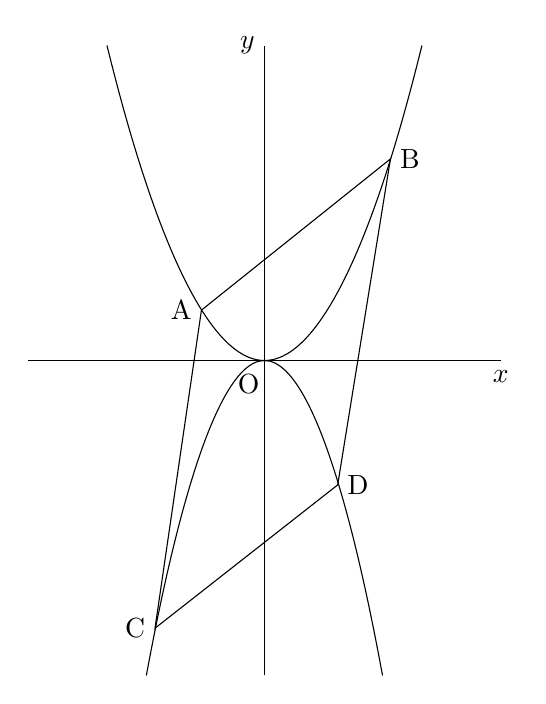
\begin{tikzpicture}
        \draw(-3,0)--(3,0) node[below] {$x$};
        \draw(0,-4)--(0,4) node[left] {$y$};

        \draw (-2,4) parabola bend(0,0) (2,4);
        \draw (-1.5,-4) parabola bend(0,0) (1.5,-4);
        \node at (-0.2,-0.3) {O};
        \coordinate (A) at (-0.8,0.64);
        \coordinate (B) at (1.6, 2.56);
        \coordinate (C) at (-1.39, -3.4);
        \coordinate (D) at (0.93, -1.58);

        
        \draw (A) node[left] {A}--(B)node[right] {B}--(D)node[right] {D}--(C)node[left] {C}--cycle;
        
      \end{tikzpicture}
    \end{center}
  \end{multicols}
  \vspace{3cm}
  
\item $\triangle$ABCにおいて, AD : DB = 1 : $x$となる点Dを辺AB上にとる. 辺BCの中点をMとし, 2つの線分AM,\ \ CDの交点をEとする.

  $\triangle$ABCの面積が$\triangle$ADEの面積の12倍であるとき,\ \ $x$の値は, $x=$ \nbox{5} である.
\end{enumerate}

\newpage

\noindent \fbox{\LARGE {\bf 2}}\hspace{10pt} AB = 6cm,\ \ BC = 8cm,\ \ CA = 10cmの$\triangle$ABCがある.

2点P,\ \ Qは, 点Aを同時に出発し, $\triangle$ABCの周上をそれぞれ以下の規則にしたがって動く.
\begin{center}
  \begin{tabular}{|l|}\hline
    P : A$\to$C$\to$B$\to$A$\to$C$\to$B$\to$Aの順に,\ \ 毎秒2cmの速さで2周する.\\ 
    Q : A$\to$B$\to$C$\to$Aの順に,\ \ 毎秒1cmの速さで1周する. \\ \hline
  \end{tabular}
\end{center}

\begin{multicols}{2}
  右の図のように, $\triangle$ABCが直線PQによって三角形と四角形に分けられるとき, 三角形の方の図形を$F$とする.

  このとき, 次の\ncircle{6} 〜 \ncircle{8} の \ebox \ にあてはまる数を求めなさい.

  \begin{center}
    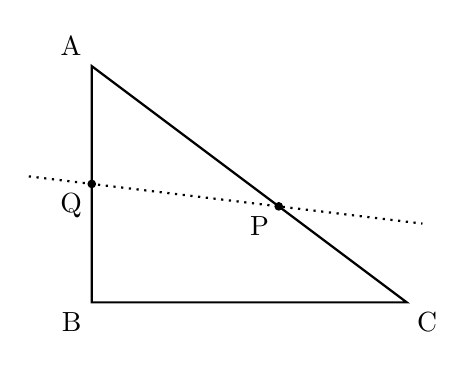
\begin{tikzpicture}
      \draw[name path = T, thick] (0,0) node[below left] {B} -- (4,0) node[below right] {C} -- (0,3) node[above left] {A} -- cycle;
      \draw[name path = L, dotted, thick] (-0.8, 1.6)--(4.2,1);

      \path[name intersections = {of = T and L}];

      \fill(intersection-1) node[below left] {P} circle[radius=0.055];
      \fill(intersection-2) node[below left] {Q} circle[radius=0.055];
    \end{tikzpicture}
  \end{center}
\end{multicols}

\begin{enumerate}[(1)]
\item $F$の面積がはじめて$\triangle$ABCの面積の半分となるのは, 2点P,\ \ QがAを出発してから \nbox{6} 秒後である. \\[4cm]
\item $F$の面積が5cm${}^{2}$となるのは全部で \nbox{7} 回あるが, 最後にそうなるのは, 2点P,\ \ QがAを出発してから \nbox{8} 秒後である.
\end{enumerate}

\newpage

\begin{multicols}{2}
  \noindent \fbox{\LARGE {\bf 3}}\hspace{10pt} 長さ$\sqrt{10}$cmの線分ABを直径とする円の周上に, AC = BCとなる点C,\ \ および点Dを右の図のようにとる. また,\ \ Cを中心としてDを通る円とDAの延長との交点をEとすると, AE=3cmであった.

  このとき, 次の \ncircle{9} ,\ \ \ncircle{10} の \ebox \ にあてはまる数を求めなさい.

  \begin{center}
    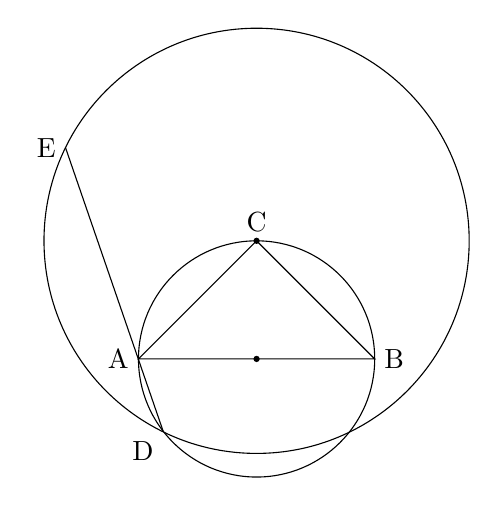
\begin{tikzpicture}
      \draw (0,0) circle[radius=1.5];
      \draw (0,1.5) circle[radius=2.7];

      \draw (-1.5,0) node[left] {A}--(0,1.5)node[above] {C}--(1.5,0)node[right] {B}--cycle;
      \fill (0,0) circle[radius=0.04];
      \fill (0,1.5) circle[radius=0.04];

      \draw ($(244:2.7)+(0,1.5)$) node[below left] {D} --($(154:2.7)+(0,1.5)$) node[left] {E};
    \end{tikzpicture}
  \end{center}
\end{multicols}
\begin{enumerate}[(1)]
\item 線分CDの長さは,\ \ CD = \nbox{9} cmである.\\[5cm]
\item Dから線分BCに垂線DFを引くと, 線分DFの長さは, DF = \nbox{10} cmである.
\end{enumerate}

\newpage

\noindent \fbox{\LARGE {\bf 4}}\hspace{10pt} 下の図のように, 4つの二等辺三角形と5つの正方形を面とする立体 O--ABCDEFGHが,\ \ 面EFGHを底面として平面$P$上に置かれている.

辺ABの長さは8cm,\ \ Oから平面$P$までの距離は24cmである.

辺BCの中点をMとする. 直線MEに平行な光線をこの立体にあてたところ, 平面$P$上にこの立体の影ができた.

このとき,\ \ 次の \ncircle{11},\ \ncircle{12} の \ebox \ にあてはまる数を求めなさい. 

\begin{center}
  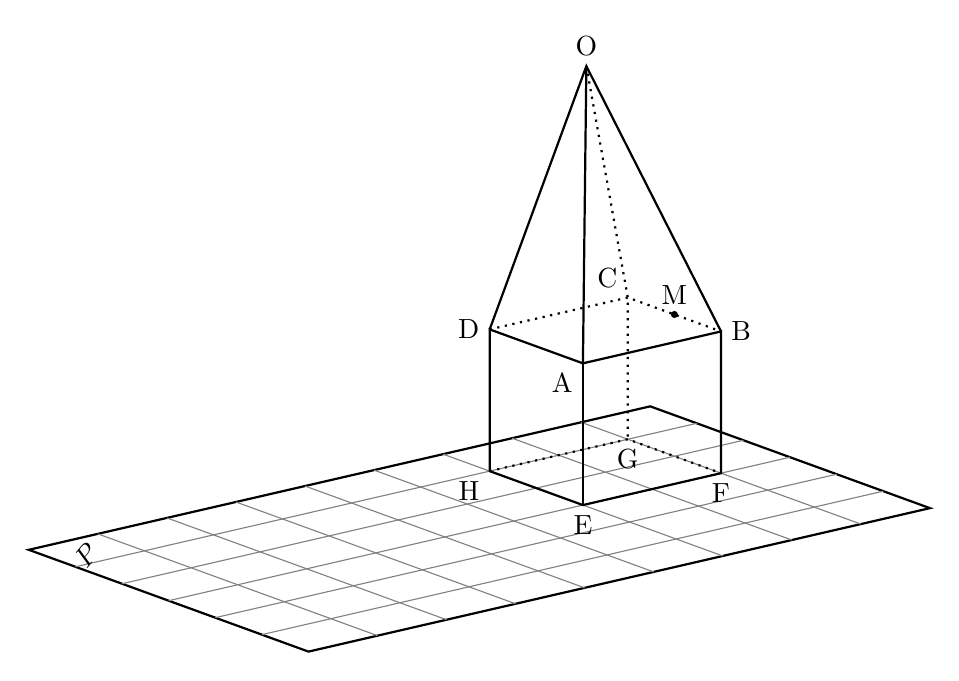
\begin{tikzpicture}[scale=0.9]
    \draw[thick] (0,0)--(160:4.2)--($(160:4.2)+(13:9)$)--(13:9)--cycle;
    \draw[draw=gray] (160:0.7)--($(160:0.7)+(13:9)$);
    \draw[draw=gray] (160:1.4)--($(160:1.4)+(13:9)$);
    \draw[draw=gray] (160:2.1)--($(160:2.1)+(13:9)$);
    \draw[draw=gray] (160:2.8)--($(160:2.8)+(13:9)$);
    \draw[draw=gray] (160:3.5)--($(160:3.5)+(13:9)$);

    \draw[draw=gray] ($(160:4.2)+(13:1)$)--(13:1);
    \draw[draw=gray] ($(160:4.2)+(13:2)$)--(13:2);
    \draw[draw=gray] ($(160:4.2)+(13:3)$)--(13:3);
    \draw[draw=gray] ($(160:4.2)+(13:4)$)--(13:4);
    \draw[draw=gray] ($(160:4.2)+(13:5)$)--(13:5);
    \draw[draw=gray] ($(160:4.2)+(13:6)$)--(13:6);
    \draw[draw=gray] ($(160:4.2)+(13:7)$)--(13:7);
    \draw[draw=gray] ($(160:4.2)+(13:8)$)--(13:8);


    \coordinate (A) at ($(160:2.1)+(13:6)+(0,2)$);
    \coordinate (B) at ($(160:2.1)+(13:8)+(0,2)$);
    \coordinate (C) at ($(160:3.5)+(13:8)+(0,2)$);
    \coordinate (D) at ($(160:3.5)+(13:6)+(0,2)$);
    \coordinate (E) at ($(160:2.1)+(13:6)$);
    \coordinate (F) at ($(160:2.1)+(13:8)$);
    \coordinate (G) at ($(160:3.5)+(13:8)$);
    \coordinate (H) at ($(160:3.5)+(13:6)$);
    \coordinate (O) at ($(160:3.5)+(13:7.4)+(0,5.4)$);
    \coordinate (M) at ($(160:2.8)+(13:8)+(0,2)$);
    
    \draw[thick] (H) node[below left] {H}--(E) node[below] {E}--(F)node[below] {F}--(B)node[right] {B}--(A)node[below left] {A}--(D) node[left] {D}--cycle;
    \draw[thick] (A)--(E);
    \draw[thick, dotted] (H)--(G) node[below] {G}--(F);
    \draw[thick, dotted] (D)--(C) node[above left] {C}--(B);
    \draw[thick] (D)--(O)--(B);
    \draw[thick] (A)--(O)node[above] {O};
    \draw[thick, dotted] (O)--(C)--(G);
    \fill (M) node[above] {M} circle[radius=0.05];

    \node[rotate  around={50:($(160:2.75)+(18:0.3)$)}] at (-3.1,-1) {$P$};
  \end{tikzpicture}
\end{center}
\newpage

\begin{enumerate}[(1)]
\item 平面$P$上にできた点Oの影を点Qとするとき, 線分OQの長さは, OQ = \nbox{11} cmである.\\[3cm]
\item この立体から四角すいO -- ABCDを取り除くと,\ \ 影の面積は \nbox{12} cm${}^{2}$だけ小さくなる.
\end{enumerate}

\newpage
\noindent \fbox{\LARGE {\bf 5}}\hspace{10pt} ある商品は単価が$a$円で,\ \ $b$個買うごとにもう1個おまけとしてもらえる($a$,\ \ $b$は正の整数).

\begin{center}
  \begin{tabular}{|l|} \hline
    例えば, $a=300$,\ \ $b=7$の場合\\
     単価が300円で,\ \ 7個買うごとにもう1個おまけとしてもらえる.\\
     30個購入すると支払金額は9000円で,\ \ おまけ4個含めて合計34個手に入る\\ \hline
  \end{tabular}
\end{center}
この商品を購入するための支払金額が1400円のとき,\ \ おまけを含めて30個手に入ることができた. このとき, 次の \ncircle{13},\ \ \ncircle{14} の\ \ebox \ にあてはまる数を求めなさい. ただし, 消費税は考えないものとする.

\begin{enumerate}[(1)]
\item 単価として考えられる$a$の値をすべて求めると, $a=$ \nbox{13} である.\\[5cm]
\item この商品を購入するための支払い金額が$c$円のとき,\ \ 1個以上のおまけを含めて合計10個手に入れることができた.

  支払い金額として考えられる$c$の値をすべてを求めると,\ \ $c=$ \nbox{14} である.
\end{enumerate}
\newpage
\thispagestyle{empty}
 
\newpage
\newpage
\thispagestyle{empty}
 
\newpage

\end{document}